%\begin{frontmatter}



%\title{Tuning properties of strongly correlated materials by means of strong laser pulses}% Force line breaks with \\
% \title{Post-Floquet engineering of electronic phase transitions by intense laser pulses}
\chapter{Strongly correlated Kramers-Henneberger solid}
\label{chap:KH_solid}
Strong laser electric fields exert forces on an electron comparable to forces binding the electron to an atomic core. Surprisingly, 
such strong fields do not always destroy the atom, but may rather create new bound electronic states residing in a new potential generated by the combined action of the laser field and the core. This so-called "Kramers-Henneberger atom" has recently been observed experimentally, settling decades of debate regarding its existence. 
Here we show that similar novel electronic structures can appear in strongly correlated solids. In our system, the effective potential generated by the laser-induced many-body dynamics traps the electrons, converting metallic into an insulating phase. The electron interaction is crucial to establish this Kramers-Henneberger solid. After the pulse is over the system remains in a state of high electronic temperature, which still has insulating (or rather a bad metallic) properties.
Our finding demonstrates new ways of manipulating phases 
of correlated systems with strong, non-resonant low-frequency 
fields, opening a new regime of "post-Floquet" engineering of strongly correlated systems. 



\section{Introduction}

Light is a powerful and versatile tool for controlling the properties of quantum systems. Exquisite control over light fields, available today, opens an opportunity to shape electronic states by
tailoring the light field, aiming to obtain "properties on demand" \citep{Basov}. 
Already at modest laser intensities, simple non-resonant shifts of atomic energy levels offer an extraordinary control tool, leading to optical traps, optical lattices, tweezers, \cite{Gao_1} etc. At higher intensities, the concept of a "dressed atom" embodies the appearance of new light-induced Floquet states, 
representing "matter + light" hybrid states with sidebands separated by the photon energy. 
These have led to new phenomena, from 
efficient laser cooling leading to 
Bose-Einstein condensation, to electromagnetically induced transparency and related phenomena, to Floquet engineering of quantum matter, e.g. using light to turn a trivial insulator into a topological \cite{Oka_Aoki_1,Kitamura_AR_2019,Huebener_1}. 
The Floquet states for time-periodic modulations are a temporal analog of the Bloch states for spatially periodic potentials.

At still higher laser intensities, the photon-counting inherent 
in the frequency-domain Floquet picture loses its simplicity -- 
too many photons are constantly exchanged between the field and the system. A welcome alternative is offered by the time-domain picture, which explicitly incorporates
the sub-cycle response of charges to the oscillating electric field. 
One example pertinent to our work is the so-called Kramers-Henneberger (KH) atom, where an intense laser field dominates the electron motion \cite{Popov_1,Henneberger_1,Gavrila_1}. The electron oscillates as nearly free so that the field-free electronic density is changed completely. 
It acquires a characteristic double-peak structure, 
with the peaks concentrated near the turning points of the 
oscillatory trajectory. The atomic core keeps the electron from drifting away, and the strongest attraction
arises when one of the two turning points is positioned 
near the core, leading to the formation of long-lived states
with a characteristic double-peaked structure.
The emergence of the Kramers-Henneberger atom leads to 
spectacular effects, from
accelerating neutral atoms at rates $\sim 10^{15}$m/s$^2$ in 
intense laser fields, to the exponential amplification of visible radiation generated
during propagation of intense infrared light in dense gases,
at the frequencies absent in the spectrum of the field-free 
gas \cite{Matthews_1}.
\begin{figure}[h!]
\begin{minipage}[h]{0.5\linewidth}
\center{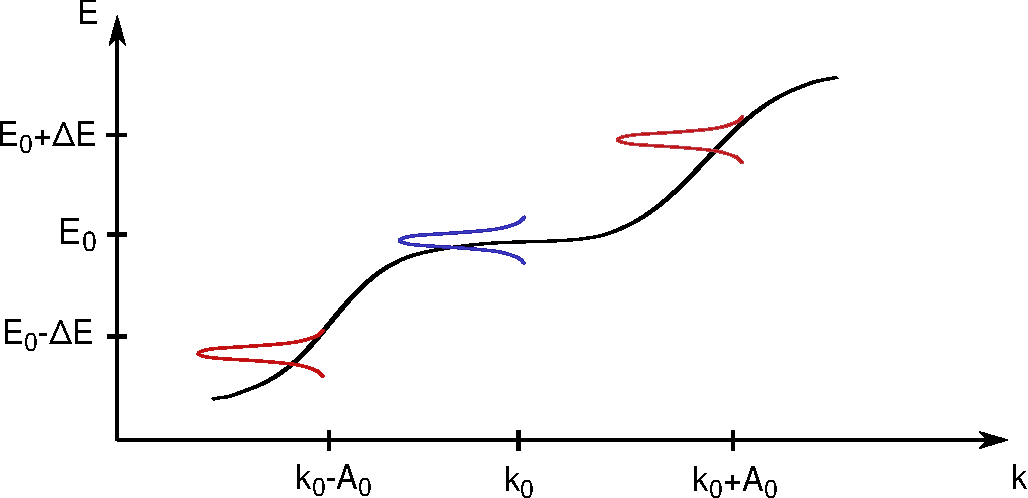
\includegraphics[width=1\linewidth]{Chapters/KH_solid/Band_sketch_1_1.pdf}} (a) \\
\end{minipage}
\hfill
\begin{minipage}[h]{0.5\linewidth}
\center{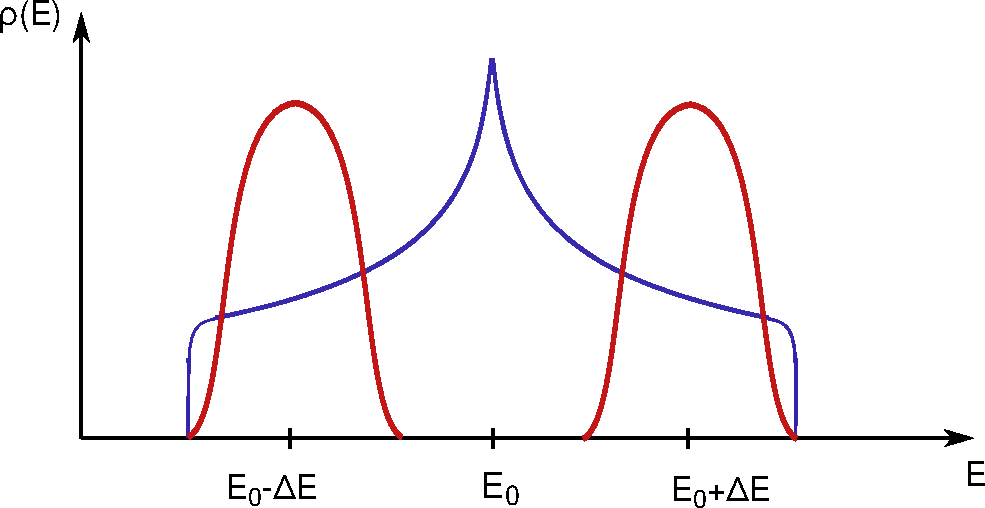
\includegraphics[width=1\linewidth]{Chapters/KH_solid/DOS_sketch_2_1.pdf}} (b) \\
\end{minipage}
\caption{Schematic band structure of square lattice. Pulse with vector potential amplitude $A_0$ drive the electrons with initial momentum $\bf k_0$ from high-density region $\text{E}_0$ to regions with momentum $\bf k_{0} \pm A_0$ and energy $\text{E}_{0}\pm\Delta\text{E}$.}
\label{BandPulse}
\end{figure}

Now we can question what will happen if we turn from an atom to electrons in solids. Fig.\ref{BandPulse} sketches the qualitative idea of extending the KH
perspective to a correlated solid modeled as a half-filled tight-binding electron model with the 
hopping rate $t_{ij}$ on a square lattice with the Hubbard-type (on-site) electron-electron repulsion $U$.
The field-free system is in the correlated metallic phase\cite{RevModPhys.68.13}, below a Mott metal-insulator transition, with the van Hove singularity 
in the density of states at the Fermi level (with the crystal momentum 
${\bf k}_0=0$, Fig.~\ref{BandPulse}a).
As the laser is turned on, it induces a current and drives the 
electrons away from the van Hove singularity to the turning
points along the dispersion curve ${\bf k}_{0} \pm {\bf A}_0$ and energy $\text{E}_{0}\pm\Delta\text{E}$ 
where
${\bf A}_0=F_0/\omega$ the amplitude of the field vector-potential
(Fig.~\ref{BandPulse}a) and $F_0, \omega$ being the field amplitude and
frequency, respectively, while $\Delta\text{E}$ defined by complicated combinations of correlation effects, a band dispersion and pulse parameters.


%This motion already in the non-interacting case has the potential to 
%transform the charge distribution from the 
%single peak near the van Hove
%singularity at the Fermi level into a double-peaked structure 
%near the turning points of the electron 
%trajectory (Fig.~\ref{BandPulse}b). 

%To induce similar modification in a 
%correlated Hubbard system and convert its metallic
%phase into insulating, the interaction with the laser field 
%should lead to the strong reduction of the 
%effective hopping rate $t_{ij}$ in the dressed system.
%This could change the system from the metallic to
%the Mott-insulating state, stabilizing 
%the insulating gap and the doubly-peaked charge distribution 
%imposed by the laser-driven motion (similar to Fig.~\ref{BandPulse}b) and moving the 
%system into an insulating state. 


%In the Floquet formalism, such transition was observed in dynamical mean-field theory and high-frequency expansion\cite{PhysRevB.93.144307,PhysRevB.99.019902}. We will discuss here experimentally realised cases of low-frequency pulses which cannot be treated in the Floquet scheme [see Sec. \ref{beyond_Floquet}].   

The mathematical analogy with the Kramers-Henneberger atom is 
as follows. The KH atom is described by transforming the 
Hamiltonian into the reference frame moving with a free electron,
${\bf r}\rightarrow{\bf r}+{\bf a}(t)$, where ${\bf a}(t)$ describes
laser-driven oscillations of the free electron.
This transformation removes the standard laser-matter interaction 
term in the Hamiltonian while modifying the electron-core interaction potential $U(\bf r)$ to
$U_{\rm KH}({\bf r},t)=U({\bf r}+{\bf a}(t))$.
The new potential exactly incorporates the dominant, laser-induced component of electron dynamics. Next, one expands 
$U_{\rm KH}({\bf r},t)$ in Fourier series.
The zero-frequency term $U^{(0)}_{\rm KH}({\bf r})$, 
which averages $U_{\rm KH}({\bf r},t)$ over the laser cycle, 
is the new effective potential describing the slow
dynamics and the 
bound states of the new system. Other 
Fourier components $U^{(N)}_{\rm KH}({\bf r})\exp(-iN\omega t)$ are responsible
for transitions between the new states. 
In lattices, the analogue of the KH-transformation is 
the Peierls substitution \cite{Peierls1933}, which moves 
the light-matter interaction term into the time-dependence of the 
hopping parameter between cites $i,j$,
\begin{equation}
t_{ij}(t)=t_{ij}\exp(-i{\bf R}_{ij}\cdot {\bf A}(t)),
\end{equation}
with ${\bf R}_{ij}$ the vector connecting the cites and ${\bf A}(t)$
the laser vector-potential. The zero-order term 
in the Fourier expansion of $t_{ij}(t)$, which for
$A(t)=A_0\cos\omega t$ is $t^{(0)}_{ij}
=t_{ij}J_0({\bf R}_{ij} {\bf A}_0)$, is the renormalized hopping rate
(here $J_0(x)$ is the zero-order Bessel function, 
$A_0=F_0/\omega$ is the amplitude of the vector potential along [11] direction in the present case, 
$F_0$ is the electric field amplitude). 
For one-electron systems, this reduction of the hopping rate leads to the well-known coherent destruction of tunneling \cite{Dunlap1986}. 

In spite of the analogy to the KH atom, the cycle-averaged electronic structure in a solid without interactions would in general not give rise to a two-peak structure as illustrated in Fig.~\ref{BandPulse}, because a hopping renormalization in all directions implies only an overall bandwidth renormalization. The essential difference to the atom is that in solid, the spectrum emerges from a superposition of delocalized momentum states such as shown in Fig.~\ref{BandPulse}. Nevertheless, we will demonstrate below the double-peaked charge distribution imposed by the laser-driven motion can be established when the field effect cooperates with the electron interaction. In correlated systems, where the interplay of the hopping rate and the on-site interaction determines the many-body state, even modest reduction in the effective hopping rate can change the system from metallic to Mott-insulating state \cite{RevModPhys.86.779}. Hence, the interaction should cooperate with the field to turn a system of delocalized electrons into a KH solid.


In the Floquet formalism, such transition was observed in dynamical mean-field theory and high-frequency expansion \cite{PhysRevB.93.144307,PhysRevB.99.019902}. We will discuss here experimentally realized cases of low-frequency pulses 
far from the off-resonant limit, 
which cannot be treated in the Floquet scheme.

%In correlated
%systems, where the interplay of the hopping rate and 
%the on-site interaction determines the many-body state, 
%even modest reduction in the effective hopping rate 
%%Mott-insulating state \cite{RevModPhys.86.779}. 
% , stabilizing 
% the insulating gap and the double-peaked charge distribution 
% imposed by the laser-driven motion (Fig.1b) and moving the 
% system into an insulating state

Note that, just like the 
KH-atom does not have to be described solely with 
the cycle-average potential $U^{(0)}_{\rm KH}({\bf r})$, 
the reduction of the hopping rate does not have to be
described solely with 
the cycle-average $t^{(0)}_{ij}$. In general, 
for 
laser frequencies the reduction 
occurs already on the sub-cycle scale\cite{PhysRevB.85.155124} as soon as the laser-induced bias $F_0a_0$ between the neighboring lattice sites ($a_0$ is the lattice constant) becomes comparable to the 
corresponding next-neighbor hopping rate $t_1$; such
sub-cycle perspective becomes particularly relevant 
for the relatively low-frequency fields 
$\omega \ll W, U$, where $W=8t_1$ is the width of the 
first Hubbard band. 

There are, of course, fundamental differences of the KH solid to laser-dressed atoms. Strong laser pulses in metals typically induce a large excitation density, which itself can have a substantial effect on the spectrum in correlated electrons. While there have been proposals to use the field-induced localization of electrons to enhance specific interaction effects in Mott insulators,\cite{dasari2019revealing,Werner_2015} where the electrons are already localized, it is therefore unclear how the KH atom emerges in a system of initially delocalized electrons. Furthermore, while light-induced effects in atoms disappear as soon as the light is turned off, the excitations in the solid can imply a persistent modification of the electronic structure. In insulators or gapped systems, this photo-excitation can generate non-thermal metastable states \cite {PhysRevLett.110.136404,PhysRevB.91.245153}. In metals, excitations typically thermalize within only few hopping times, even in the vicinity of the Mott transition \cite{PhysRevLett.120.166401, PhysRevLett.103.056403}. It should be emphasized that in correlated systems this huge increase in electron temperature can transform a metal into a bad metallic or insulating-like state with a pseudo-gap, and hence imply a modification of the electronic structure which is typically not accessible in equilibrium (because the lattice cannot by heated to correspondingly high temperatures).

%However, there is a fundamental difference between 
%laser-dressed systems such as atoms and a 
%strongly correlated system.
%In atoms, light-induced states disappear as soon as the 
%light is turned off. Here, however, the interplay of a strong  
%laser field and correlated dynamics generates
%a metastable state surviving after the end of the laser pulse.
%The presence of long-lived non-thermal states, which 
%do not relax to the thermal ones after the driving field is switched off \cite {PhysRevLett.110.136404,PhysRevB.91.245153}, is an important property 
%of correlated systems. Intense laser field allows us 
%to access such transient states, which are 
%inaccessible via adiabatic or thermal pathways \cite{RevModPhys.86.779}. 

Highly non-perturbative interaction involving a vast number of photons and generating new system properties after the end of the pulse offers control beyond Floquet engineering.  
In contrast to phonon-driven transitions \cite{Cavalleri_2011}, 
our mechanism is purely electronic, with the effect arising
within a fraction of the cycle of the driving laser field.

\section{Kramers-Henneberger solid}

To demonstrate this qualitative idea quantitatively, 
we consider a two-dimensional, half-filled square 
Fermi-Hubbard lattice interacting with intense,
linearly polarized field. In contrast to previously studied 
Bethe- or hypercube-lattices \cite{PhysRevLett.106.236401,PhysRevB.91.245153} or one-dimensional chains\cite{Rui}, here the field can be applied either along one of the lattice directions, obtaining a quasi one-dimensional system (studied e.g. by Silva et al. \cite{Rui}), or along the diagonal, obtaining the situation similar to the Bethe-lattice or infinite-dimensional hypercube, but with realistic two-dimensional band electron dispersion, including the van Hove singularity at the Fermi level and sharp band step at the edges. To treat the non-perturbative 
time-dependent problem, we used the non-equilibrium 
extension \cite{schmidt2002,RevModPhys.86.779} of 
the Dynamical Mean-Field Theory (DMFT) \cite{RevModPhys.68.13}.
The algorithm and its realization are described in [Sec. \ref{section:Hubbard_model} and \ref{section:NE_DMFT} of \autoref{chap:Non_mb_th}] \cite{PhysRevB.81.115131}, for technical details. The method was benchmarked 
against exact diagonalization of one-dimensional finite 
chain used in Ref.~\cite{Rui}, see Sec.~\ref{Benchmark}.

The implementation is based on the NESSi simulation package for non-equilibrium Green's functions \cite{nessi}.

The key optical observable encoding the 
dynamics of the system is
the coherent light emission generated 
by the laser-induced current. The current operator is defined as
\begin{equation}
\label{Current}
{\bf j}(t)=-\dfrac{ie}{V}\sum_{{\bf k} \sigma} v_{\bf k} G_{{\bf k},\sigma}^{<}(t,t),
\end{equation}
where $V$ is the volume, $e$ - charge of electron (equal to 1 in our units)\cite{PhysRevB.84.035122}
. 
Detecting coherent light emitted by the system 
offers excellent diagnostic of the underlying 
charge dynamics. Modern light characterization methods 
such as e.g. 
frequency-resolved optical gating (FROG) \cite{Trebino_1997, Kane_1993} 
or spectral shearing interferometry \cite{Iaconis_1998} allow one to characterize both 
spectral amplitude and spectral phase of
the emitted light.
The resulting time- and frequency-resolved  
spectrograms (known as the FROG spectrograms)  
represent the window Fourier (e.g. Gabor) transform 
favored by theorists and allow one to reconstruct the 
generated current and the underlying charge dynamics with
temporal resolution limited only by the inverse spectral 
width of the generated emission, i.e. often 
far better than one cycle of the driving field. These techniques
are particularly well developed in the IR and visible frequency
range, which we focus on here, see Ref.\cite{RupertHuber_2015} for a 
a striking example of about 1 fs temporal resolution in
the experimental measurement of high harmonic
emission induced by THz field. 
% To generate 
% the emission spectrograms, we use
% the Gabor transform of the current. 


% The spectral function is calculated as
% \begin{equation}
% G^{ret}(w,t)=-\frac{1}{\pi}Im\int ds e^{iws}G^{ret}(t,t-s).
% \label{Gret}
% \end{equation}

% The population density is calculated as
% \begin{equation}
% G^{<}(w,t)=-\frac{1}{\pi}Im\int ds e^{iws}G^{<}(t,t-s).
% \label{Gles}
% \end{equation}

We use hopping parameters for undoped 
LaCuO$_4$ (LCO), with the lattice constant $a_{0}=3.78\AA$ and
$t_1=0.43$~eV \cite{Markiewicz}. 
The width of the
non-interacting band dispersion is $W=8t_1=3.44$~eV.  
We set the value of Hubbard $U=2.5$ eV,  
close to the estimate of Ref.\cite{Delannoy}.
We use few-cycle pulses, such as
shown in Fig.~\ref{Fig:Light_induced_transition}a, where it has a central wavelength of $\lambda=1500$~nm ($\omega=0.827$~eV) and duration of 7.6 fs (full width at half-maximum, FWHM), with
total simulation time 32.8 fs. We found no significant frequency dependence for the dynamical localization processes 
described below in the studied range 
$\omega=0.4...16$~eV. Here we focus on the 
relatively low-frequency regime $\omega \ll W,U$
but kept $\omega\geq t_1$ and present results for
$\lambda=1500$~nm and $\lambda=3000$~nm.
The pulse polarization was parallel to the lattice diagonal ([11] direction), to ensure that both lattice directions are
equally affected by the laser field. 

% Although 0.827~eV pulse frequency is chosen for the present calculations, the system behavior stays the same with lowering pulse central frequency down to at least $\omega=0.4$~eV, so the lower frequency pulses could also be used in order to decrease laser flux and concomitant sample damage approaching the equal peak vector potential.
% We found no significant frequency dependence for the dynamical localization processes described in this section, at least in the range 
% $\omega=0.4...16$~eV. 
%The peak value of the vector potential, that is one of the key values determining the system behavior, is varied in the range $A_{max} = 0.25...4.9$, that corresponds to electric field strength of order of $8*10^{8}$~V/m to $2*10^{10}$~V/m for lattice parameter equal to $a_{0}=3.78\AA$, lattice constant for $CuO_2$ plane of LCO. These values correspond to 0.36~$mJ/cm^2$ to 71.2~$mJ/cm^2$ pulse fluence for $150\times200 \mu m$ focus size.
% // for 800 nm; The data for the pulse above is also available, no significant difference found.

One of the key parameters governing system response is the maximal value of vector potential
${A}_{0}$. For  
$\omega=0.827$~eV the range 
${A}_{0} = 0.37,..., 2.3$ corresponds to the laser field intensity range from
$I_0=8.3 \times 10^{10}$W/cm$^2$ 
($F_0=0.08$ V/A) 
to $I_0=3.5 \times 10^{12}$W/cm$^2$ 
($F_0=0.5$ V/A). The voltage across the 
unit cell approaches the hopping rate, $a_0F_0 \simeq V_1$, at  
$I_0\simeq 1.6 \times 10^{11}$W/cm$^2$
($F_0\simeq 0.1$ V/A). Thus, in our system
fields at the level of $F_0\simeq 0.1$ V/A enable 
strong modification of the effective hopping rate and
thus can alter the structure of the correlated system.  
The relation between the maximal pulse intensity $I_0$ and the maximal strength of the pulse electric field $F_0$
is given by $I_0 = \frac{c \epsilon_0 F_0^2}{2}$, where c is the speed of light and $\epsilon_0$ is the permittivity of free space.
%The case of the electric field parallel to one of the lattice directions %([100] direction)
%({\it y-polarization}) 
%was also considered, however the model became quasi one-dimensional, giving results similar to ones discussed in Ref.~\cite{Rui}: no occupation inversion, no change of the $U_{eff}$ sign. 

% \begin{figure}
% 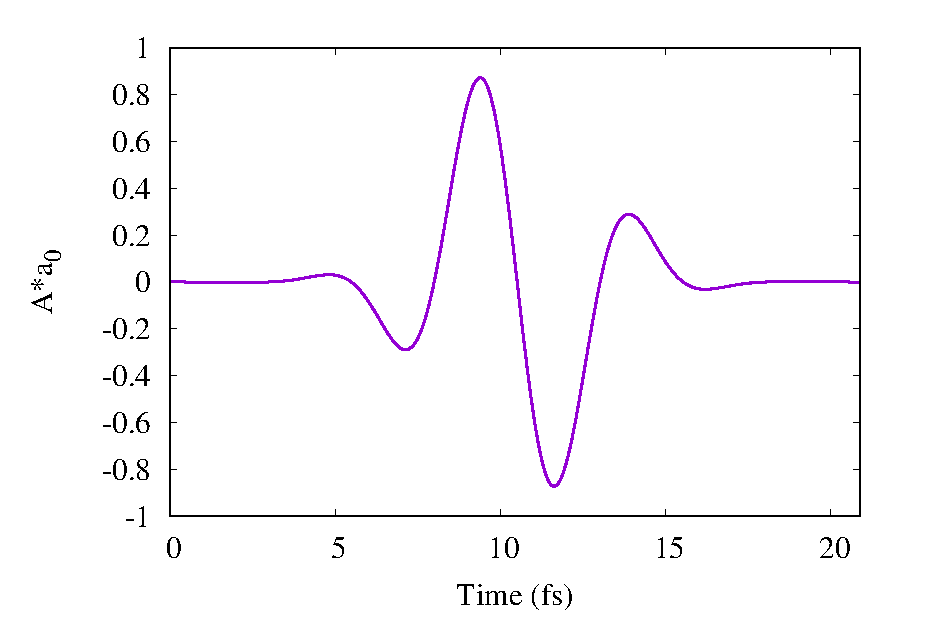
\includegraphics[width=1.0\linewidth,angle=0]{Pulse1p5A1.eps}
% \caption{The vector potential for the Gaussian pulse 
% with carrier $\omega=0.827$~eV, and $A_{0}\times a_0=1$.}
% \label{Pulse1p5A1}  
% \end{figure}

Our results are summarized in Figs.~4.2-4.4. 
Fig.~\ref{Fig:Light_induced_transition}a shows the electric field of the 
pulse carried at 1500 nm, while Fig.~\ref{Fig:Time_resolved_energy}b shows
the electric field of the pulse carried at 
3000 nm. The dynamical response is very similar in
these two cases.

Fig.~\ref{Fig:Light_induced_transition}(b-d) show the time-dependent population
densities [Eq.\eqref{Spectr_R_L_2} in Sec. \ref{subsection:Spectral_function} of \autoref{chap:Non_mb_th}] for increasing field
strength.  
Transfer of spectral weight from the van Hove singularity 
(located at the zero energy $E=0$) 
\begin{figure}[h!]
\begin{minipage}[h]{0.5\linewidth}
\center{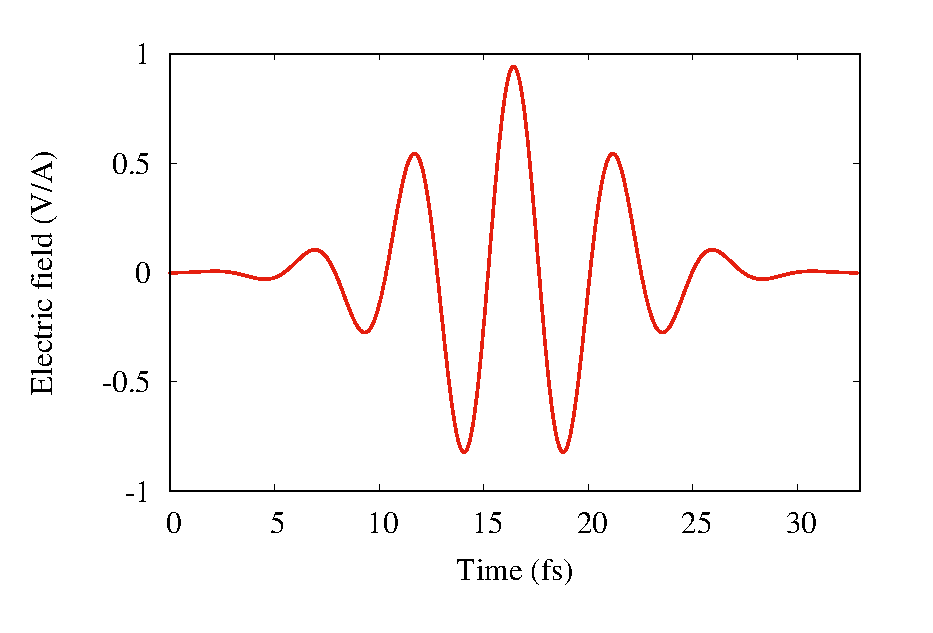
\includegraphics[width=1\linewidth]{Chapters/KH_solid/E_32.eps}} (a) \\
\end{minipage}
\hfill
\begin{minipage}[h]{0.5\linewidth}
\center{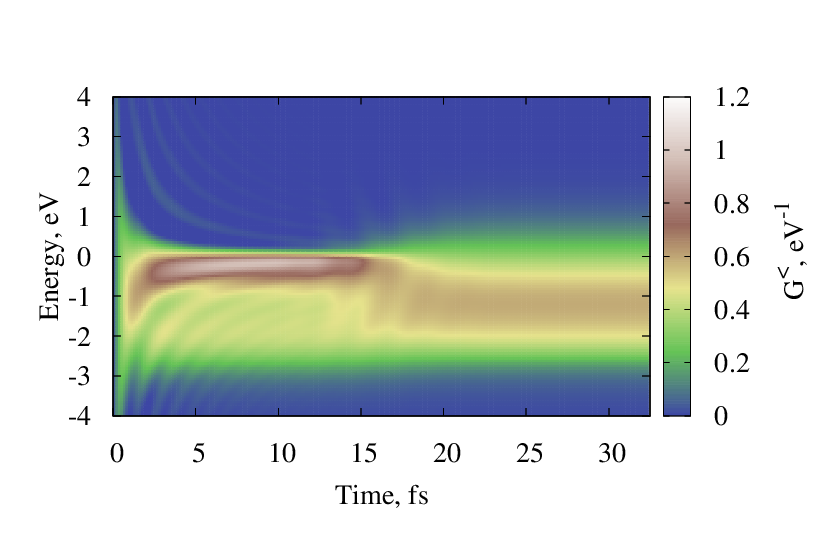
\includegraphics[width=1\linewidth]{Chapters/KH_solid/3d_les_E_1_10_9.png}} \\(b)
\end{minipage}
\begin{minipage}[h]{0.5\linewidth}
\center{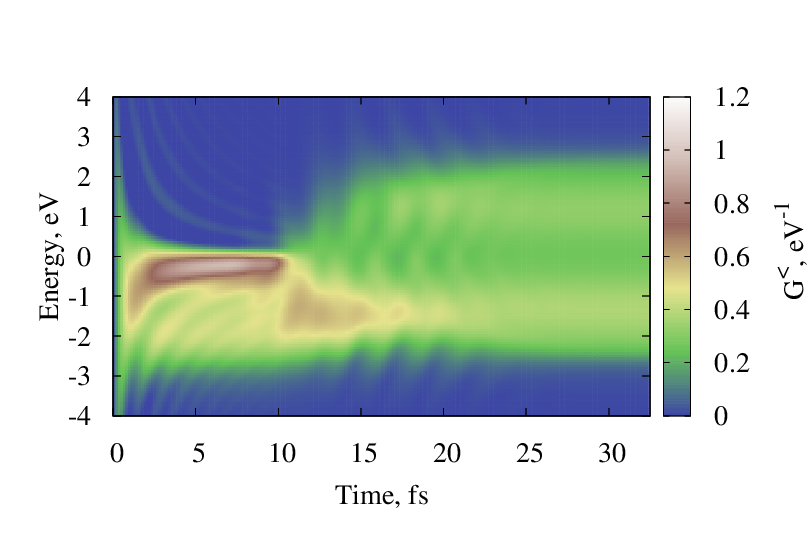
\includegraphics[width=1\linewidth]{Chapters/KH_solid/3d_les_E_5_10_9.png}} (c) \\
\end{minipage}
\hfill
\begin{minipage}[h]{0.5\linewidth}
\center{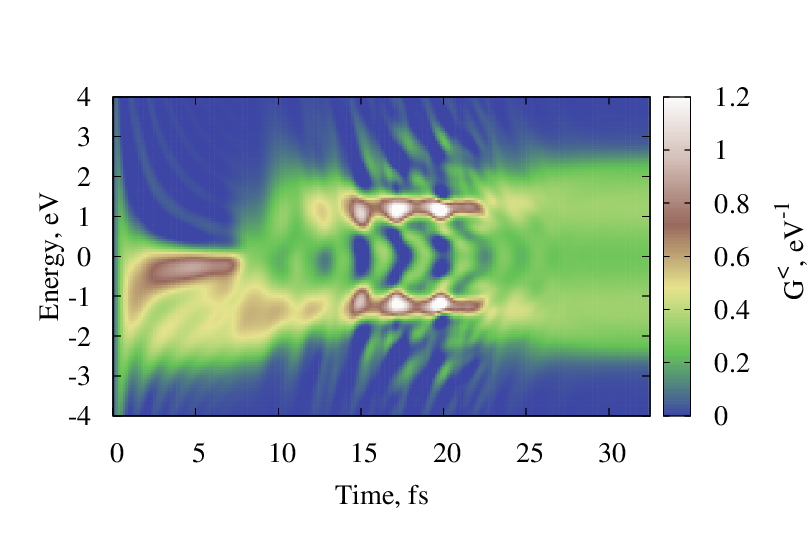
\includegraphics[width=1\linewidth]{Chapters/KH_solid/3d_les_E_2_10_10.png}} \\(d)
\end{minipage}
\caption{Light-induced transition from the metallic to 
the Mott-insulating state. 
(a) The electric field for the Gaussian pulse carried at 
$\omega=0.827$~eV used in the simulations. 
(b-d) Time-dependent population density for 
%$E_{max}=8*10^{8}$V/m (a),
the field amplitude $F_0=0.1$ V/A (b), 0.5 V/A (c), and 2.0 V/A (d).}
\label{Fig:Light_induced_transition}
\end{figure}
to the Hubbard bands becomes prominent 
as soon as the field approaches 0.1 V/A. 
The response is manifestly sub-cycle, within about 1 fs. 
At lower fields (Fig.~\ref{Fig:Light_induced_transition}b) the system stays predominantly in the lower Hubbard band during the whole interaction. 
It also does not return to the original distribution near the 
van Hove singularity once the pulse is over.
At higher fields (Fig.~\ref{Fig:Light_induced_transition}c), 
we see substantial population transfer from the lower 
to the upper Hubbard band (situated at $E=1.25$ eV) 
with the spectral gap opening. Blurring the graphs of occupied states within 5 femtoseconds is due to the lack of data for the Fourier transform from time to frequency.
The sub-cycle nature of the nonlinear response remains evident, 
including the splitting of the population between the upper and the lower bands as the electric field rapidly goes through its maxima, with the transient return of small spectral weight near zero energy as the electric field goes through zero. 
Crucially, the double-band Mott-type structure
survives well after the end of the pulse, 
Fig.~\ref{Fig:Light_induced_transition}(b-d), signifying 
the transition from a metallic to an insulating-type structure, 
induced by the laser field and stabilized by correlation.
The gap formation is confirmed by Fig.~\ref{Fig:Time_resolved_energy}, which shows that
the total energy in the system increases in steps synchronized with the instantaneous maxima in the laser electric field. 
This is true for both $\lambda=1500$ nm and $\lambda=3000$ nm
drivers. Note that the steps for both frequencies are
very similar in height, showing that the transitions are
in the quasi-static low-frequency regime.
\begin{figure}[h!]
\begin{minipage}[h]{0.5\linewidth}
\center{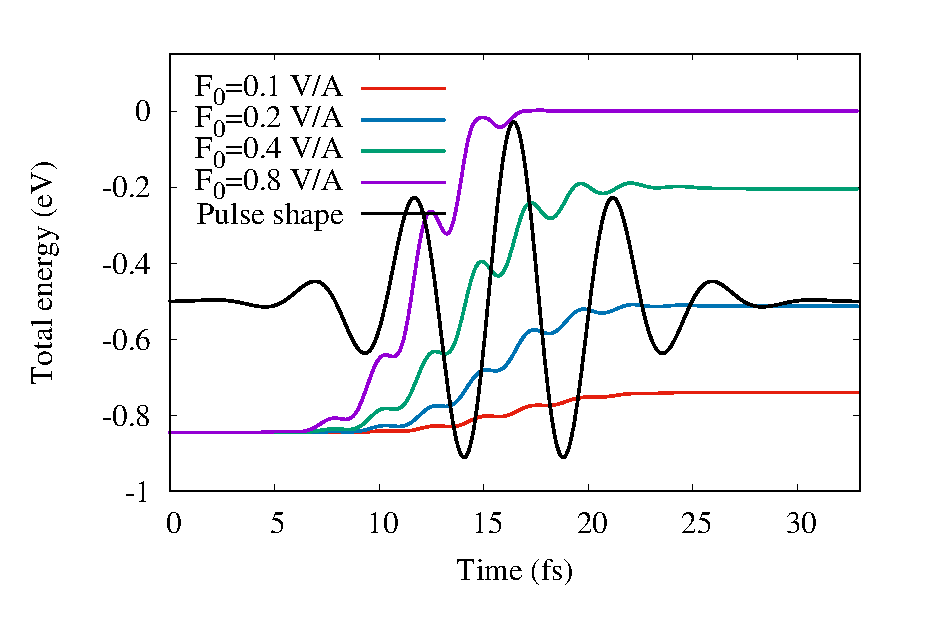
\includegraphics[width=1\linewidth]{Chapters/KH_solid/Etot_w192.eps}} (a) \\
\end{minipage}
\hfill
\begin{minipage}[h]{0.5\linewidth}
\center{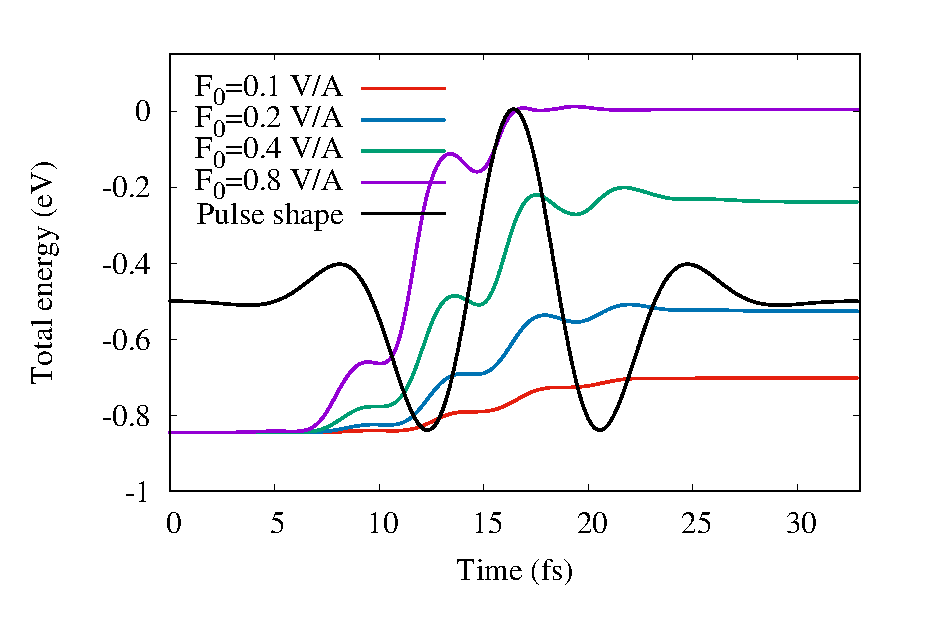
\includegraphics[width=1\linewidth]{Chapters/KH_solid/Etot_w0961.eps}} (b) \\
\end{minipage}
\caption{Time-resolved energy absorption by the 
driven system with different peak field strengths (from $F_0=0.1$ V/A to $F_0=0.8$ V/A)
for 1500 nm (a) and 3000 nm (b). For guide we also show the shape of electric field.}
\label{Fig:Time_resolved_energy}
\end{figure}

Such frequency-independent step-wise behavior is characteristic of the tunneling limit in non-adiabatic excitation across a bandgap, be
it in an atom or a solid. In this regime the 
instantaneous transition amplitude across the 
energy gap is $A\propto \exp(-F_{\rm thr}/F(t))$. Here 
$F(t)$ is electric field with Gaussian envelop (Fig.~\ref{Fig:Light_induced_transition}a),
$F_{\rm thr}$ is the characteristic "threshold" field.
In a Mott insulator with a gap $\Delta$, 
$F_{\rm thr}\simeq \Delta /2\xi$ \cite{Oka_2003,Oka_2005,Oka_2010,Oka_2012}, where
$\xi\sim a_0$ is the correlation length. In our system,
an estimate for $F_{\rm thr}$ 
along the lattice direction is $F_{\rm thr}\sim U/2a_0=0.33 $V/A,
implying the threshold electric field amplitude of $F\simeq F_{\rm thr}\sqrt{2}=0.47$ V/A along the [11] direction. This estimate
is in excellent agreement with the observed behavior of 
$E_{\rm tot}(t)$, where the  
fields with amplitude $F>0.4-0.5$ V/A lead to 
saturation of excitation within a field cycle.
\begin{figure}[h!]
 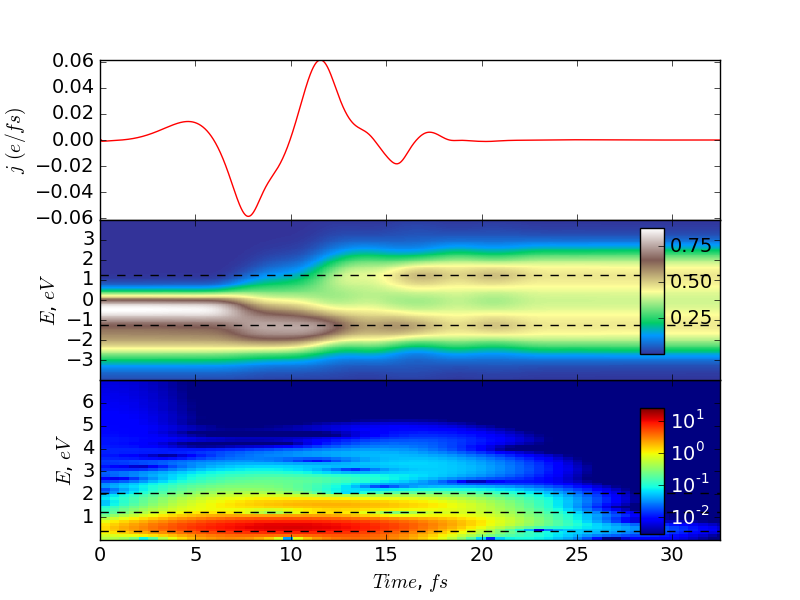
\includegraphics[width=0.9\linewidth,angle=0]{Chapters/KH_solid/2_w_0_961.png}
\caption{Upper panel: A gaussian pulse at a central frequency $\omega=0.413$~eV, width $d=7.7$~fs, and intensity $F_{0}=0.8$~V/A, polarization along [11]. The generated current is shown in red. Middle panel: Time-dependent PES, dash lines denotes positions of Hubbard bands $\pm U/2$ (with $U=2.5$). Lower panel: Gabor transform of the current the dash line denotes position of odd $\omega$ harmonics generation in case of constant ac-field.}
\label{HHG_1}  
\end{figure}

As expected in the low-frequency regime, the
transition from the 
metallic phase to dynamical localization with
a gap is very similar for 3000 nm driver, and 
occurs as the instantaneous 
electric field exceeds $\sim 0.1-0.2$ V/A. An example
is shown in Fig.~\ref{HHG_1}, for the peak amplitude
of the driving field $F_{0}=0.8$ V/A.
Fig.~\ref{HHG_1}(upper panel) shows the driving electric field
(blue) and the generated current (red). Fig.~\ref{HHG_1}(middle panel) shows 
the time-resolved formation of the 
lower Hubbard band and the gap, as tracked by 
$I(\omega, t_p)$. In Fig.~\ref{HHG_1}(middle panel), the gap opens around 7-8 fs, 
when the instantaneous field reaches $\sim 0.1-0.2$ V/A. 
The excitations across the bandgap into the upper Hubbard 
band occur near the maxima of the instantaneous 
field, most notably at $\sim 12-13$ fs and $\sim 16-17$ fs.
Excitation is accompanied by 
suppression of the current, which is fully quenched 
at $\sim 18$ fs, when the excitation of the upper Hubbard band 
saturates and the insulating state is established. 
\begin{figure}[h!]
 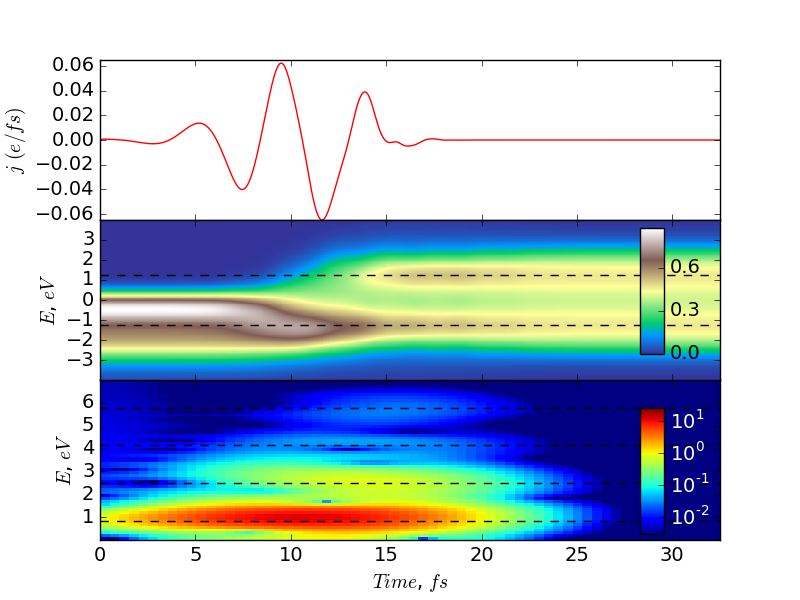
\includegraphics[width=0.9\linewidth,angle=0]{Chapters/KH_solid/2_w_1_92.png}
\caption{Upper panel: A gaussian pulse at a central frequency $\omega=0.827$~eV, width $d=7.7$~fs, and intensity $F_{0}=0.8$~V/A, polarization along [11]. The generated current is shown in red. Middle panel: Time-dependent PES, dash lines denotes positions of Hubbard bands $\pm U/2$ (with $U=2.5$). Lower panel: Gabor transform of the current the dash line denotes position of odd $\omega$ harmonics generation in case of constant ac-field.}
\label{HHG_2}  
\end{figure}

The time-resolved optical signatures of charge dynamics are
encoded in the induced current and the 
coherent emission it generates (given 
by the Fourier transform of the current). As we have
already pointed out, time-resolved characterization of
the emission is feasible with about 1 fs accuracy.
The emergence of the gap and the step-wise injection of
charge across the gap inevitably lead to bursts
of current near the field maxima. Their Fourier transform
produces characteristic odd harmonics (dominated by
3rd and fifth), often referred to
as the Brunel harmonics \cite{Burnett_1989}. Thus, we expect that
efficient harmonic generation would start
with the formation of the Mott gap and cease when the excitation across the gap is saturated. 

The harmonics generation in Fig.~\ref{HHG_1} not coincide with odd frequencies of the pulse with limitation low-frequency external field by the Gaussian envelope. In Fig.~\ref{HHG_2} situation changing due to increasing the pulse frequency.


These expectations
are confirmed in Fig.~\ref{HHG_1}(bottom panel), which shows the FROG-type 
spectrogram of the emission, obtained using the Gabor transform
with a 3-fs (full width at half-maximum) Gaussian window. Indeed, the spectrogram contains clear information about the laser-induced reshaping of
the many-body state and the formation of the Mott gap. 
When the system is in the metallic state, the field
generates a strong current at the driving frequency. 
Harmonics are synchronized with the formation of
the gap and cease when light-induced step-wise transitions
across the bandgap are saturated. 



\section{Summary}

Modification of the electronic properties
of quantum systems with light opens new opportunities for
using light to tailor the ultrafast electronic response. 
Our work brings the strong-field concepts developed for
atomic systems in the context of strongly correlated
metals. 

%Altering the effective 
%potential for the electron motion with strong pulse light we 
%convert the system from a metallic state to the state
%with a Mott gap. 

We show how many-body correlations help to establish the field-induced transient insulator out of delocalized electrons. After the pulse, the system is transferred into a state of high electron temperature, which is inaccessible under equilibrium conditions and remains more insulating than the initial state, with a pseudo-gap. 
The dynamics in time-domain is 
resolved via harmonic generation spectroscopy, which 
encodes the formation of the Mott gap, 
excitation dynamics across it, and the establishment 
of the insulating state. 
Our findings demonstrate the possibility of manipulating phases 
of correlated systems with strong, non-resonant  
fields in a manner that is extremely robust with respect to the specific
frequency of the driving field, with the time-domain 
mechanisms opening a new regime of "beyond-Floquet" engineering of 
strongly correlated systems.

\FloatBarrier
\section{\label{beyond_Floquet}Appendix: Beyond-Floquet parametrization.}

To show the difference of regimes in current article calculations and high-frequency Floquet behavior we would like to demonstrate how much the dependence of the band narrowing on the magnitude of the vector potential. Here we use vector potential with [11] polarization limited by Gaussian envelope.  The mean value of the vector potential $\tilde{A}$ selected in the range from -FWHM to FWHM. Below we provide calculations for 2D square lattice with initial inverse temperature $\beta=1/T=5$ and $50 \times 50$ $k$-grid. For convenient comparison with other theoretical works all results in units of hopping. Where $t=1=0.43$eV; $U=5.81t=2.5$eV; $W=8t=3.44$eV; $\omega=1.92t=0.827$eV. 
\begin{figure}[h!]
\begin{minipage}[h]{0.5\linewidth}
\center{\includegraphics[width=1\linewidth]{Chapters/KH_solid/Intensity_of_LHB_occ_1.eps}} (a) \\
\end{minipage}
\hfill
\begin{minipage}[h]{0.5\linewidth}
\center{\includegraphics[width=1\linewidth]{Chapters/KH_solid/Width_of_LHB_occ_1.eps}} (b) \\
\end{minipage}
\caption{Dependence of intensity (a) and FWHM (b) of lower Hubbard band on the average value of vector potential $\tilde{A}$ in the middle of the pulse.}
\label{Fig:LHB_I_W}
\end{figure}

We consider two quantities: Intensity of lower Hubbard band(LHB) (Fig.~\ref{Fig:LHB_I_W}a) and FWHM (Fig.~\ref{Fig:LHB_I_W}b) of lower Hubbard band in the middle of the pulse where the value of vector potential equal zero. Both graphs were calculated using the photoemission spectrum and were also compared with data obtained from DOS.
\begin{figure}[h!]
\begin{minipage}[h]{0.5\linewidth}
\center{\includegraphics[width=1\linewidth]{Chapters/KH_solid/E_tot_1.eps}} (a) \\
\end{minipage}
\hfill
\begin{minipage}[h]{0.5\linewidth}
\center{\includegraphics[width=1\linewidth]{Chapters/KH_solid/docc_1.eps}} (b) \\
\end{minipage}
\caption{Dependence of total energy (a) and double occupancy (b) on the average value of vector potential $\tilde{A}$ in the middle of the pulse.}
\label{Fig:E_tot_docc_KH}
\end{figure}
The purple line corresponds to the position of zeros in zero-order Bessel function $J_0(A_x)$. One can expect that in the Floquet regime intensity of LHB will be maximum at positions of $J_0(\tilde{A}_x)=0$. For high-frequency regime ($\omega=10.47$ and $\omega=20.94$) the maximum of LHB achieve $J_0(\tilde{A}_x)=0$. For low pulse frequency, the intensity of LHB ceases to be consistent with the behavior of the $J_0(A_x)$.

Fig.~\ref{Fig:E_tot_docc_KH}a,b show dependence of total energy and double occupancy on the $\tilde{A}$ in the middle of the pulse. Energy absorption is significantly lager for low frequency ($\omega=1.92$ and $\omega=5.24$) as well as the number of excitations.


\FloatBarrier
\section{\label{Benchmark}Appendix: Benchmark of IPT results and exact diagonalization}

We performed a benchmark of our IPT on square lattice to the code 
Ref. \cite{Rui}, performing exact diagonalization for the finite 12-site one-dimensional chain.
\begin{figure}[h!]
 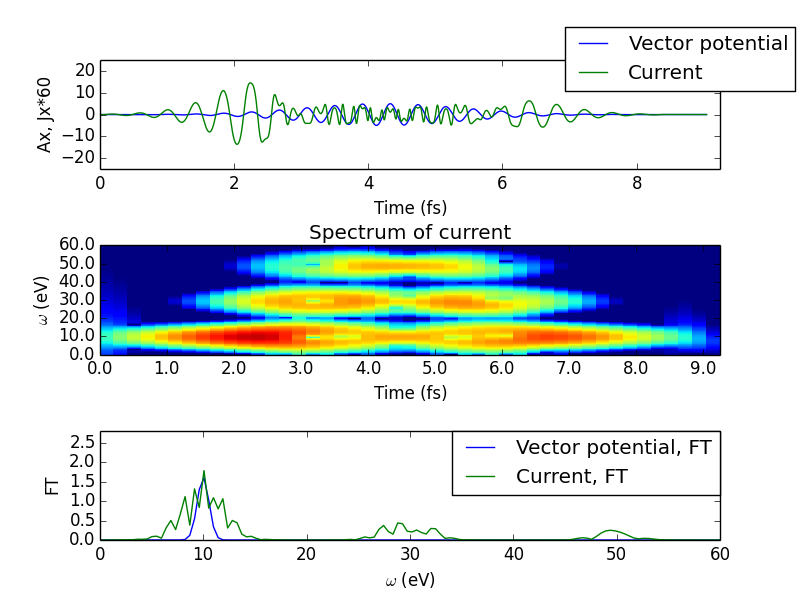
\includegraphics[width=0.9\linewidth,angle=0]{Chapters/KH_solid/HHGtestVitja.png}
\caption{Higher harmonic generation on square lattice for gaussian pulse with central frequency $\omega=10$~eV, $FWHM=3$~fs, and $A_{0}=5$, polarization along [10] direction. Upper panel: vector potential (blue) and current (green); middle panel: Gabor transform of the current; Lower panel: spectra of incoming pulse (blue) and current (green).}
\label{HHGtestVitja}  
\end{figure}
The hoppings $t=1$~eV, on-site Coulomb repulsion $U=6$~eV, pulse vector potential amplitude $A_{0}=5$, pulse FWHM is 3 fs, pulse central frequency $\omega=10$~eV. In order to compare our two-dimensional lattice model to one-dimensional chain, we choose linear pulse polarization along [10] direction and relatively large field amplitude.

Although the physics of 1D and 2D systems is different in sense of 
possibility of closed loops and additional scattering channels in two-dimensional lattice, the resulting HHG spectra are looking qualitatively similar (see Figs. \ref{HHGtestVitja} and \ref{HHGtestRui}).  
\begin{figure}[h!]
 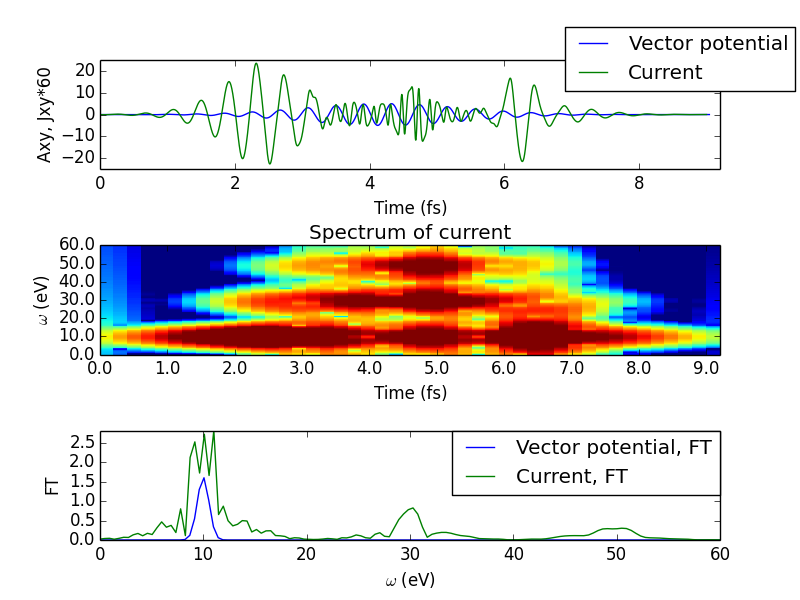
\includegraphics[width=0.9\linewidth,angle=0]{Chapters/KH_solid/HHGtestRui.png}
\caption{Higher harmonic generation on 12-sites chain for gaussian pulse with central frequency $\omega=10$~eV, $FWHM=3$~fs, and $A_{0}=5$, polarization along the chain. Upper panel: vector potential (blue) and current (green); middle panel: Gabor transform of the current; Lower panel: spectra of incoming pulse (blue) and current (green, red, cyan).}
\label{HHGtestRui}  
\end{figure}















